\chapter{Conception}
Avant de commencer à coder le projet il nous a fallut effectuer un tutoriel pour comprendre comment utiliser la bibliothèque GraphStream. Nous avons ainsi apprit à implémenter des nœuds, les relier entre eux, construire des graphes.
Une fois ce tutoriel effectué et acquis par chacun nous avons pu commencer à implémenter le projet. \newline

Il se compose des classes CustomGraph, Database et Point, deux énumérations UniteSpatiale et UniteTemporelle et enfin notre Main pour exécuter le programme.
\section{Classes}
\subsection{CustomGraph}
 La classe CustomGraph est la classe permettant de créer des graphes et de les afficher. Elle est la classe principale de notre projet.Elle est composée d'un constructeur basique qui prend en entrée une Database, une UniteTemporelle et une UniteSpatiale.
 Une méthode display() qui construit et affiche le graphe voulu en fonction des paramètres choisis.
  et une méthode toString().
\subsection{Database}
 La classe Database dispose d'un constructeur qui permet une connexion à notre base de données, une méthode logout() pour se déconnecter, une méthode createView() qui permet de créer ou remplacer une vue à partir d'une UniteTemporelle et une UniteSpatiale elle utilise la méthode getRequest() qui va générer une requête suivant l'UniteTemporelle et renverra la requête SQL associée.
 Et les deux dernières méthodes getPointsLocalisation() et getPointsFrontiere() permettant d'obtenir respectivement les points de la localisation et des villes et frontières et de les stocker dans une collection.
\subsection{Point}
Cette classe permet simplement de créé un point avec des coordonnées x et y utilisé par la suite dans les classes CustomGraph et Database.
\subsection{Enumerations}
 L'énumération UniteTemporelle est composée de MOIS, JOUR, HEURE, MINUTE et l'énumération UniteSpatiale est composée de COMMUNES et DEPARTEMENTS.
\subsection{Main}
  Notre Main qui lance le programme est composé d'un menu qui permet de choisir les paramètres voulus et enfin fait appel à la méthode display() de CustomGraph afin de construire et afficher le graphe demandé.
  \section{Diagramme de classes}
  \vfill
  \begin{figure}[ht!]
    \centering
     \caption{Diagramme de classes }
     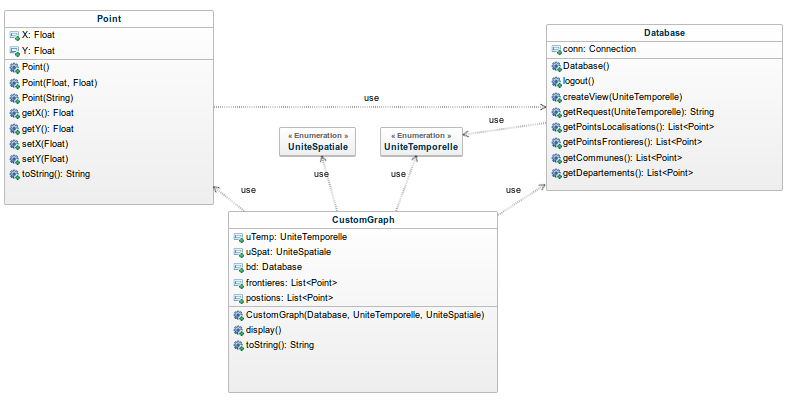
\includegraphics[scale=0.5]{RO.png}
  \end{figure}
  \vfill
